\part{Nivel de enlace}
\section{Introducción}
La capa de enlace de datos tiene que desempeñar varias funciones específicas, entre las que
se incluyen:
\begin{itemize}
  \item Proporcionar una interfaz de servicio bien definida con la capa de red.
  \item Manejar los errores de transmición.
  \item Regular el flujo de datos para que receptores lentos no sean saturados por emisores rápidos.
\end{itemize}
Para cumplir con estas metas, la capa de enlace de datos toma de la capa de red los paquetes y los encapsula en \textbf{tramas} para transmitirlos. Cada trama contiene un \textbf{encabezado}, un campo de carga útil (\textbf{payload}) para almacenar el paquete y un \textbf{terminador} o final. El manejo de las tramas es la tarea primordial de la capa de enlace de datos.

\subsection{Servicios proporcionados}
La capa de enlace de datos puede diseñarse para ofrecer varios servicios. Los servicios reales
ofrecidos pueden variar de sistema a sistema. Tres posibilidades razonables que normalmente se
proporcionan son:
\begin{enumerate}
  \item \textbf{Servicio no orientado a la conexión sin confirmación de recepción:} Consiste en hacer que la máquina de origen envíe tramas independientes a la máquina de destino sin pedir que ésta confirme la recepción. No se establece conexión de antemano ni se libera después. Si se pierde una trama debido a ruido en la línea, en la capa de enlace de datos no se realiza ningún intento por detectar la pérdida ni por recuperarse de ella.
  \item \textbf{Servicio no orientado a la conexión con confirmación de recepción:} Cuando se ofrece este servicio tampoco se utilizan conexiones lógicas, pero se confirma de manera individual la recepción de cada trama enviada. De esta manera, el emisor sabe si la trama ha llegado bien o no. Si no ha llegado en un tiempo especificado, puede enviarse nuevamente.
  \item \textbf{Servicio orientado a la conexión con confirmación de recepción:} Con este servicio, las máquinas de origen y de destino establecen una conexión antes de transferir datos. Cada trama enviada a través de la conexión está numerada, y la capa de enlace de datos garantiza que cada trama enviada llegará a su destino. Es más, garantiza que cada trama será recibida exactamente una vez y que todas las tramas se recibirán en el orden adecuado.
\end{enumerate}

\subsection{Separación de frames:}
Puesto que es demasiado riesgoso depender de la temporización para marcar el inicio y el final de cada trama, se han diseñado otros métodos:

\begin{enumerate}
  \item \textbf{Largo fijo:} Todos los paquetes tienen la misma longitud.
  \item \textbf{Conteo de caracteres}: Se vale de un campo en el encabezado para especificar el número de caracteres en la trama. Cuando la capa de enlace de datos del destino ve la cuenta de caracteres, sabe cuántos caracteres siguen y, por lo tanto, dónde está el fin de la trama. El problema con este algoritmo es que la cuenta puede alterarse por un error de transmisión. Si esto pasa, el destino perderá la sincronía y será incapaz de localizar el inicio de la siguiente trama. Incluso si el destino sabe que la trama está mal porque la suma de verificación es incorrecta, no tiene
  forma de saber dónde comienza la siguiente trama. Regresar una trama a la fuente solicitando una retransmisión tampoco ayuda, ya que el destino no sabe cuántos caracteres tiene que saltar para llegar al inicio de la retransmisión.
  \item \textbf{Flags con bit-stuffing}: El segundo método de entramado evita el problema de tener que sincronizar nuevamente después de un error, haciendo que cada trama inicie y termine con bytes especiales llamado \textbf{flags}. De esta manera, si el receptor pierde la sincronía simplemente puede buscar la bandera para encontrar el final e inicio de la trama actual. Dos banderas consecutivas señalan el final de una trama y el inicio de la siguiente. 
  
  Cuando se utiliza este método para transmitir datos binarios, como programas objeto o números de punto flotante, surge un problema serio. Se puede dar el caso con mucha facilidad de que el patrón de bits de la bandera aparezca en los datos (payload), lo que interferiría en el entramado. Una forma de resolver este problema es hacer que la capa de enlace de datos del emisor inserte un byte de \textbf{escape especial} (ESC) justo antes de cada bandera “accidental” en los datos. La capa de enlace de datos del lado receptor quita el byte de escape antes de entregar los datos a la capa de red. Esta técnica se llama \textbf{relleno de caracteres} o bit-stuffing. Por lo tanto, una bandera de entramado se puede distinguir de uno en los datos por la ausencia o presencia de un byte de escape que la antecede.
\end{enumerate}

\subsection{Detección y corrección de errores}

Los diseñadores de redes han desarrollado dos estrategias principales para manejar los errores. Una es incluir suficiente \textbf{información redundante} en cada bloque de datos transmitido para que el receptor pueda deducir lo que debió ser el carácter transmitido. La otra estrategia es incluir sólo suficiente redundancia para permitir que el receptor sepa que ha ocurrido un error (pero no qué error) y entonces solicite una retransmisión. La primera estrategia utiliza \textbf{códigos de corrección de errores}; la segunda usa \textbf{códigos de detección de errores}. 

\subsubsection{Detección de errores}
\paragraph{Bit de paridad:} La forma más sencilla. Consiste en añadir un bit de paridad al final del bloque de datos. El valor de ese bit se determina de tal forma que el código resultante tenga un número impar de unos. El receptor examina el código recibido y, si el número total es impar, supondrá que no ha habido errores. 

La utilización de bits de paridad no es infalibre, ya que los impulsos de ruido son a veces lo suficientemente largos como para destruir más de un bit.

\paragraph{Comprobación de redundancia cíclica (CRC):} Dado un bloque o mensaje de \(k\)-bits, el trasmisor genera una secuencia de \(n\)-bits denominada \textbf{secuencia de comprobación de la trama} de tal manera que la trama resultante con \(n+k\) bits, se divisible por algún número determinado. El receptor entonces divirá la trama recibida por ese número y, si no hay resto en la división, se supone que no ha habido errores.

\subsubsection{Códigos de corrección de errores}
Por lo general, una trama consiste en \(m\) bits de datos (es decir, de mensaje) y \(r\) bits redundantes o de verificación. Sea la longitud total \(n\) (es decir, \(n = m + r\)). A una unidad de \(n\) bits que contiene datos y bits de verificación se le conoce como palabra codificada de \(n\) bits.

Dadas dos palabras codificadas cualesquiera es posible determinar cuántos bits correspondientes difieren aplicando un OR exclusivo a las dos palabras codificadas y contar la cantidad de bits 1 en el resultado. La cantidad de posiciones de bits en la que difieren dos palabras codificadas se llama \textbf{distancia de Hamming}. Si dos palabras codificadas están separadas una distancia de Hamming \(d\), se requerirán \(d\) errores de un bit para convertir una en la otra.  

Para detectar \(e\) errores se necesita un código con distancia \(e + 1\), pues con tal código no hay manera de que \(e\) errores de un bit puedan cambiar una palabra codificada válida a otra. Cuando el receptor ve una palabra codificada no válida, sabe que ha ocurrido un error de transmisión. De manera similar, para corregir \(e\) errores se necesita un código de distancia \(2e + 1\), pues así las palabras codificadas legales están tan separadas que, aun con \(e\) cambios, la palabra codificada original sigue estando más cercana que cualquier otra palabra codificada, por lo que puede determinarse de manera única. 

\subsection{Protocolos de Transmición confiable}
\subsubsection{Stop \& Wait}
\begin{figure}[H]
	\centering
	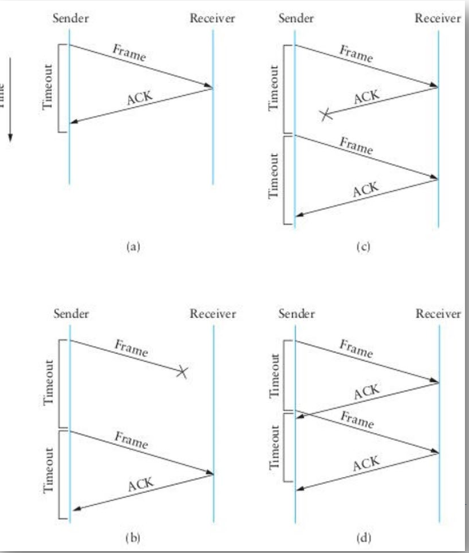
\includegraphics[width=0.65\textwidth
]{images/stop-wait.png}
	\caption[Protocolo Stop And Wait]{Protocolo Stop And Wait}
	\label{fig:stop-wait}
\end{figure}
La máquina de origen emite un único frame y espera la recepción de una confirmación (ACKnowledgment) durante un período determinado de tiempo \(t\). Mientras tanto no podrá enviar ningún otro frame.


Pueden surgir dos problemas durante la comunicación:
  
El receptor detecta algún error, entonces descartará el frame y no manda el ACK. El temporizador expira antes de la recepción del ACK y re-envía el último frame.

Por otro lado, si el frame llega correctamente y el receptor envía una ACK pero el ACK se pierde en el camino, tambien expira el temporizado y el origen vuelve a enviar el mismo frame. 
  
El destino recibe por segunda vez el frame como si fuese un frame distinto.

Para evitar este problema, los frames se etiquentan alternadamente con 0  1, y las confirmaciones positivas serán de la forma ACK0 y ACK1. Un ACK0 confirma la recepción de un frame numerada con 0 e indica que el receptor está esperando para aceptar un frame numerado con 0.

Ahora, cuando el receptor reciba dos frames con la misma numeración, podrá interpretar que está recibiendo un frame duplicado porque su ACK se perdió en el camino. En este caso, el receptor descartará el frame y volverá a mandar el ACK correspondiente.

\paragraph{Eficiencia de un protocolo:} 
Vamos a definir:
\begin{itemize}
  \item \(T_{tx}\) el tiempo de transmición de un frame (lo que tarda en ir desde el origen hasta el destino).
  \item \(RTT(F)\) el tiempo de retorno del ACK, osea el tiempo que tarda en llegar el frame al receptar sumado al tiempo que tarda en llegar el ACK al emisor original. En genaral va a pasar que \(RTT(F) = Delay\times 2\) 
\end{itemize}

El rendimiento de un protocolo \(\eta\) se define como:

\[\eta_{proto} = \frac{T_{tx}(F)}{RTT(F)}\]

\subsection{Ventana deslizante}
Aumentar la eficiencia \(eta\), implica disminuir al minimo la cantidad de tiempo que el origen se bloquea durante la espera de un ACK.

Una estrategia posible para esto es enviar varios frames seguidos, sin esperar ACKs para cada uno.
Aparece el concepto de \textbf{ventana de frames}: en una ventana se envía una cierta cantidad de frames. Esto resulta en una definición diferente para la eficiencia:

\[\eta_{proto} = \frac{T_{tx}(V)}{RTT(F)}\]

donde \(T_{tx}(V)\) es el tiempo de transmición de una ventana.

Sea \(V_{tx}\) la velocidad de transmición, definimos la capacidad de volumen de un canal \(C_{vol} = V_{tx}\times Delay\) como la cantidad de bits que entran en un canal de manera simultáneas sin saturarlo. Con esto, podemos calcular el \textbf{Sliding Window Size (SWS)} de la siguiente manera:

\[SWS = \frac{V_{tx}\times RTT(F)}{|Frames|} \text{ frames}\]

Al comenzar la comunicación, la máquina origen manda \(SWS\) frames al máquina destino. Y espera a recibir el ACK del primer frame enviado. Cuando esto sucede, el origen manda el siguiente frame de la secuencia.

Por cada ACK recibido, el origen va mandando de a uno los frames restantes siempre y cuando el último frame enviado pertezca a una ventana que contenga al frame del último ACK recibido.

\begin{itemize}
  \item \textbf{ACKs Acumulativos:} Si un ACK se pierde, el receptor descarta todos los paquetes hasta que reciba el paquete que está esperando. Esto va a provocar que se produzca un timeout en el emisor del primer paquete perdido y de todos los siguientes, por lo que volverá a enviar todos los frames de nuevo desde el último ACK recibido.
  \item \textbf{ACKs Selectivos:} El receptor recibe y se guarda todos los frames que van llegando. Supongamos que recibe el frame \(i\) con errores. Cuando llega el frame \(i + 1\) responde al receptor con un NAK\(i\). Esto le indica al emisor que si bien recibió el último paquete enviado, hubo un error en el frame anterior y tiene que reenviarlo.
  
  El receptor sigue aceptando frames y respondiendo con ACK\(i-1\) hasta que consigue correctamente el frame perdido. En este momento, responde con un ACK\(j\) donde \(j\) corresponde con el último frame que recibió sin error.
\end{itemize}

Los frames están enumerados de manera cíclica desde 1 hasta \(SWS + RWC\) donde \(RWC\) es el tamaño de la ventana de recepción y se define de la siguiente manera:

\[
  RWC = \begin{cases}
    SWS & \text{si hay ACKs Selectivos} \\
    1 & \text{si hay ACKs Acumulativos}
  \end{cases}
\]

\begin{figure}[H]
	\centering
	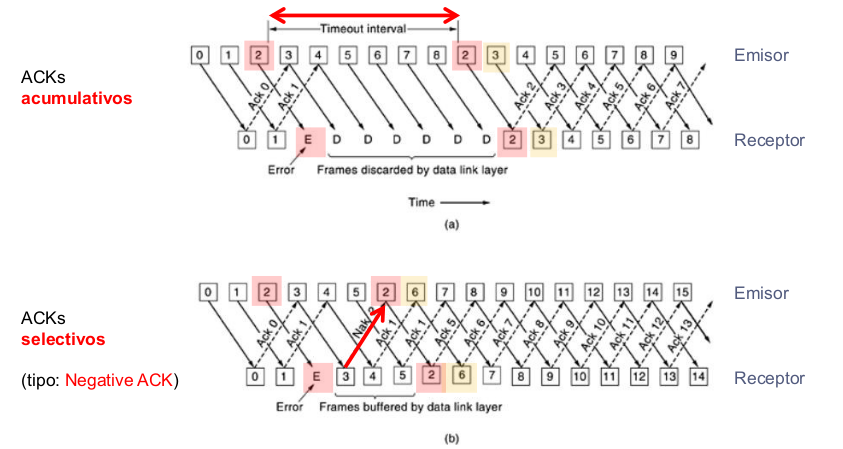
\includegraphics[width=\textwidth
]{images/sliding-window.png}
	\caption[Protocolo Sliding Window]{Protocolo Sliding Window}
	\label{fig:sliding-window}
\end{figure}